\documentclass[11pt]{article}

\usepackage[utf8]{inputenc} % Required for inputting international characters
\usepackage[T1]{fontenc} % Output font encoding for international characters

%\usepackage{mathpazo} % Palatino font
\usepackage{graphicx}
\usepackage{amsmath}
\usepackage{amsfonts}
\usepackage{wrapfig}

\begin{document}

%----------------------------------------------------------------------------------------
%	TITLE PAGE
%----------------------------------------------------------------------------------------

\begin{titlepage} % Suppresses displaying the page number on the title page and the subsequent page counts as page 1
	\newcommand{\HRule}{\rule{\linewidth}{0.5mm}} % Defines a new command for horizontal lines, change thickness here
	
	\center % Centre everything on the page
	
	%------------------------------------------------
	%	Headings
        % Full name of the issuing organization and its logo
	%------------------------------------------------
	%------------------------------------------------
	%	Logo
	%------------------------------------------------
	
	\vfill\vfill
	
\includegraphics[width=0.5\textwidth]{logo.png} % Include a department/university logo - this will require the graphicx package
	 
	%----------------------------------------------------------------------------------------
	
	
        \vspace{1cm}
	\HRule\\[0.4cm]
        \textsc{\Large Advanced Reactors and Fuel Cycles Group}\\
        {\Large Technical Report Series}\\ % Report Series
	
	{\large ARFC-NPRE-17-00}\\ % Report number

	
	%------------------------------------------------
	%	Title
        % Title of the report
	%------------------------------------------------
	
	\HRule\\[0.4cm]
	
	{\huge\bfseries Inception Neural Networks for Isotope Identification}\\[0.4cm] % Title of your document
	
        %{\LARGE\textit{Subtitle}}\\[0.4cm] % Subtitle
	\HRule\\[1.5cm]
	
	%------------------------------------------------
	%	Author(s)
	%------------------------------------------------
	
	\begin{minipage}{0.4\textwidth}
		\begin{flushleft}
			\large
			\textit{Prepared for:}\\
			\textsc{American Nuclear Society}\\ % 
                        \textsc{Contract} NN-NNNN\\ % 
                \end{flushleft}
	\end{minipage}
	~
	\begin{minipage}{0.4\textwidth}
		\begin{flushright}
			\large
			\textit{Prepared by:}\\
			Samuel \textsc{Dotson}\\ %
			Mark \textsc{Kamuda}\\ %
			Prof. Kathryn \textsc{Huff} %
		\end{flushright}
	\end{minipage}
	
	% If you don't want a supervisor, uncomment the two lines below and comment the code above
	%{\large\textit{Author}}\\
	%John \textsc{Smith} % Your name
	
	%------------------------------------------------
	%	Date
	%------------------------------------------------
	
	\vfill\vfill\vfill % Position the date 3/4 down the remaining page
	
	{\large\today}\\ % Date, change the \today to a set date if you want to be precise
        \vfill
	%------------------------------------------------
	%	Place
	%------------------------------------------------
	{\large Urbana, IL}\\ % Place
        {\large Department of Nuclear, Plasma, and Radiological Engineering\\
        University of Illinois at Urbana-Champaign}\\ % Issuing Instituion
	
	
	
	\vfill % Push the date up 1/4 of the remaining page
	
\end{titlepage}

%----------------------------------------------------------------------------------------

\section{Introduction}
The development of algorithms that can accurately identify the isotopic sources of low-resolution gamma-ray 
spectra is an important advancement in  current spectroscopy workflow (Sullivan, 2010).
Previous work has shown that artificial neural networks can be used to perform isotope identification (Cite: [3], [4], [5]). This paper introduces a new feature to the existing architecture of the Artificial Neural Network for Spectroscopic Analysis (ANNSA) package. This new feature is known as an Inception Neural Network (INN). An INN implements inception layers that consist of wide convolutional layers with several filters, rather than the typical single-filter layer in a simple convolutional neural network (CNN).
This paper also demonstrates improved methods for simulating spectra to better emulate the background radiation found in real measurements. 
The features of a gamma-ray spectrum vary depending on the full width at half max (FWHM) of the photopeaks. 
Simultaneously applying multiple filters of different sizes allows an INN to capture more features during a single layer than a CNN. 
We hypothesize that an INN will also be robust to changes in background radiation thereby generalizing the ANNSA framework to more scenarios. 
We compare the accuracy of an INN to a simple CNN to determine if the improvement in accuracy is enough to warrant the increased computational complexity. 
Finally, new training data will be obtained through simulations with GADRAS-DRF (Mitchell and Harding, 2014) software.


\begin{figure}[h]
\centering
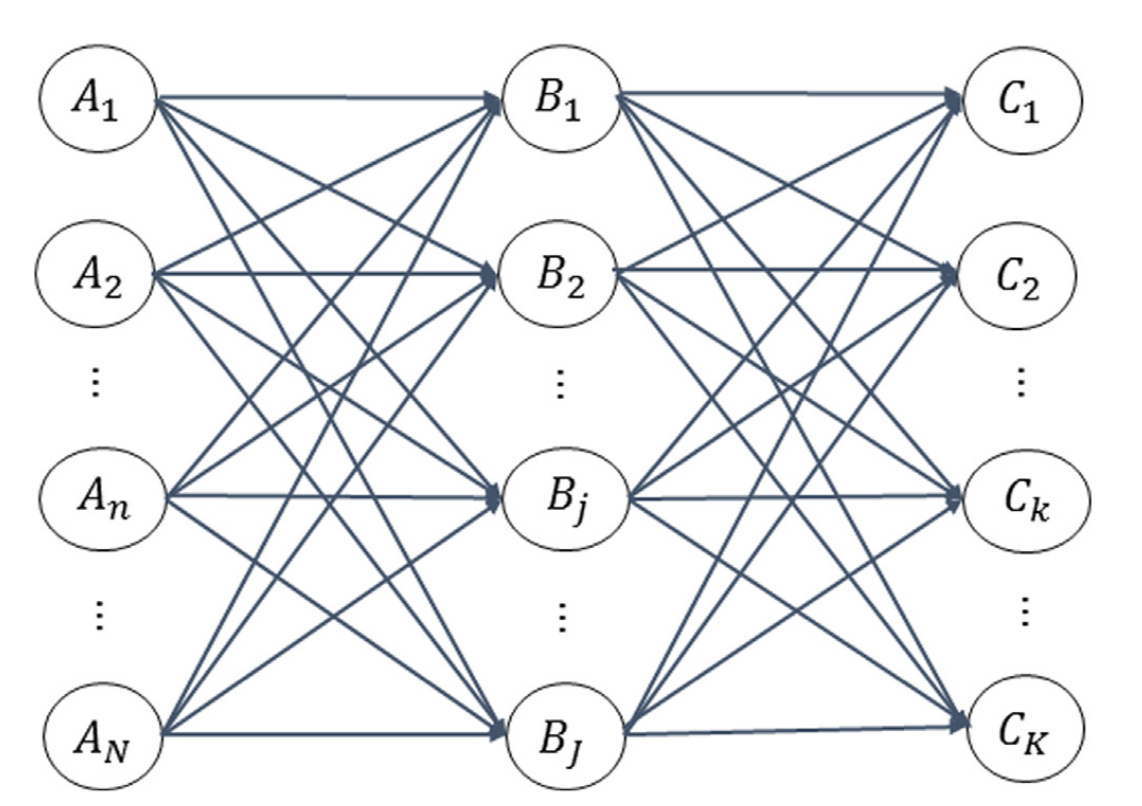
\includegraphics[width=0.5\textwidth]{dense-layer-figure.png}
\caption{An arbitrary neural network that maps values with weights (arrows).}
\label{fig:dense-nn}
\end{figure}
\begin{figure}[h]
\centering
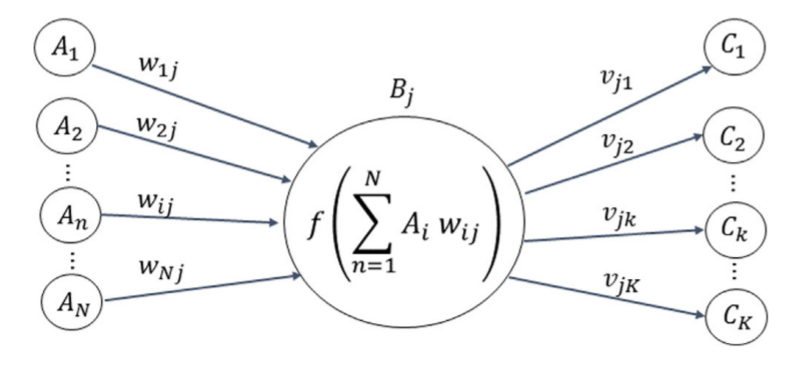
\includegraphics[width=0.5\textwidth]{neuron-figure.png}
\caption{A single neuron being passed through an activation function, $\textit{f}$.}
\label{fig:neuron}
\end{figure}


\section{Theory -- Artificial Neural Networks}

An artificial neural network (ANN) is a function that maps values from ${\mathbb{R}}_{N}$ to ${\mathbb{R}}_{K}$ by mimicking biological 
neurons. Examples of an arbitrary neural net and a single neuron are shown in Fig. 1 and Fig. 2. The 
sum of the inputs times the weights pointing to a neuron are passed through an activation function.
In this paper it is a rectified linear unit,

\begin{equation}
Relu = argmax(0, x).
\end{equation}
The result is used as the input for the next layer, as shown in Fig. 2. 
An ANN may be trained by iteratively updating the weights of a network that minimizes an error function, $E$. 
The weights are updated through back propagation by taking the derivative of $E$ with respect to the weights. 
The error function minimized during training of the INN is cross-entropy,

\begin{equation}
E = -\sum_{c}^{M}y_{o,c}\ln{p_{o,c}}.
\end{equation}


Eq. 2 is the cross-entropy for multiclass classification, where there are more than two possible labels 
for a given input. M is the total number of labels for a given model, in this case it corresponds to 29 
radionuclides (ANSI, 2015). Variable $y_{o,c}$ is binary, indicating whether observation, o, has the correct label, c. 
Variable $p_{o,c}$ is the probability that o is a member of c. The complete INN model is shown in Fig. 3 and Fig. 4. 
The input for the INN is a 2”x2” NaI spectrum of 1024 channels and the final output is a softmax given by,

\begin{equation}
softmax(z_j) = \frac{\exp(z_j)}{\sum_{k=1}^{k}}.
\end{equation}


\begin{figure}[h]
    \centering
    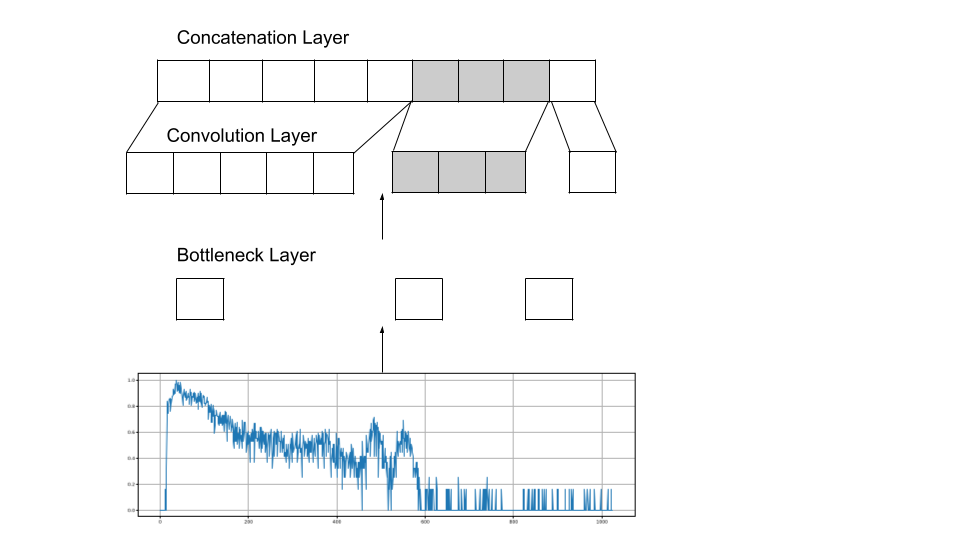
\includegraphics[width=\textwidth]{inn-layer_figure.png}
    \caption{A gamma spectrum shown as the input for the first inception layer.}
    \label{fig:inn-layer}
\end{figure}
\begin{figure}[h]
    \centering
    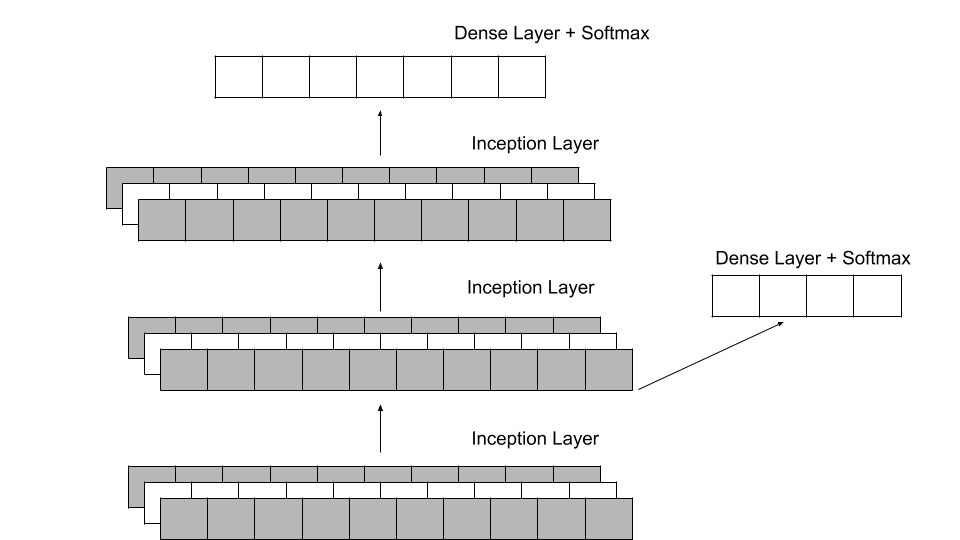
\includegraphics[width=\textwidth]{inn-full-figure.png}
    \caption{A zoomed out example of a full inception neural network.}
    \label{fig:inn-full}
\end{figure}

The input data is passed through three inception layers and, after flattening, the output is passed to a dense layer which gives the final softmax output. 
Each inception layer has a bottleneck, a convolution, and a concatenation (Szegedy, et. al, 2014).
The bottleneck is performed to reduce the computational complexity before large convolution filters are applied. 
A large filter can be factorized into several smaller filters thereby reducing the number of required multiplications. 
The convolution layer uses filters to select features of a spectrum that have local spatial significance, but no long-range relationships. 
Once the convolution has been done with several filters in parallel the outputs of each of those convolutions are concatenated into a single tensor that is passed to the next inception layer, or dense layer if the last layer has been reached. 
Just like a typical CNN (Fig. [5]), the final step after feature identification, is classification. 
Classification is performed by using a dense, or fully connected, layer that learns weights that correspond to a probability for a certain label. 
In this case, the corresponding labels are radioactive isotopes.


\section{Methods}
\subsection{Training set creation}
It is infeasible to obtain enough real measurements to properly train a neural network. 
Thus all of the datasets used to train the neural network here were simulated using GADRAS-DRF (Mitchell and Harding, 2014). 
The 29 isotopes in the dataset are based on the American National Standards Institute performance criteria for handheld instruments for the detection and identification of radionuclides, ANSI N42-34-2015 (ANSI, 2015). 
Previous work (Kamuda, et. al 2018) used a uniform distribution of background isotopes and a constant average count of 65 counts per second (cps) for the background. 
Simulating background radiation in this manner is insufficient for training a neural network to be robust against background variations and thus cannot be generalized to real conditions. 
We are updating the simulation protocol to increase the variability in background conditions. New simulated data will include random noise in a range of 40 to 200 cps. 
We believe this range is realistic for background radiation.
\subsection{Network Structure and Hyperparameters}
A neural network can memorize training sets resulting in overtraining and a misidentification of novel data. 
This is especially true for an INN, whose weights are difficult to tune with simple back propagation.
To solve this problem during training, we include an intermediate softmax output that allows for error corrections before the entire forward pass is complete. 
This branch is ignored during prediction, but offers a way to prevent overtraining. 
In the fully connected layer, dropout regularization forces the neural network to learn newpathways. 
Hyperparaemters can be used to optimize performance and prevent overfitting of the model.
There is no way to know which hyperparameters will influence the model before training, so a random hyperparameter search is performed to find a set of hyperparameters that are close to ideal (Bergstra and Bengio, 2012). 
For CNN structures, like the INN, hyperparameters include the number and sizes of convolutional filters, and the number of nodes and dropout rate for the fully connected layer. 
\subsection{Benchmark Techniques}
In order to compare the efficiency of these two neural networks and the effectiveness of updated datasets, we will train each network twice. 
Once by reusing data from previous work (Kamuda, et. al,  2018) and again with the improved datasets. 
This will allow us to identify if accuracy improved more due to a sophisticated algorithm or the advance is attributable to better training data, or some combination thereof. 
The INN will demonstrate a satisfactory improvement over the CNN if the amount of time required to train the network results in an equivalent reduction in variance for predictions. 
For concreteness, a 10 percent increase in training time should correspond to a 10 percent, or greater, decrease in the variance for the INN when compared with the training time and variance of the CNN.

\section{Conclusion}

In this study, we compare the accuracy of two neural networks, a convolutional neural network with two convolutional layers and an inception neural network with three inception layers, for identifying radioactive isotopes in low-resolution gamma-ray spectra. 
We hypothesize that the INN would exhibit an increase in robustness commensurate to its computational complexity and that training the neural networks with larger and varied datasets will also improve its robustness. 
Improvements to the identification of isotopes present in a sample of radioactive material will have important implications for national security and nuclear nonproliferation.


%\begin{thebibliography{References}
%\bibitem{}
%\bibitem{}
%\bibitem{}
%\bibitem{}
%\bibitem{}
%\bibitem{}
%\end{thebibliography}


\end{document}

